\chapter{Expérience simple d'interaction}
\label{Chapitre : Première exprérience simple d'interaction}
\thispagestyle{fancy}

\section {Présentation de l'expérience}
\label{Section : 6.présentation de l'expérience}
Cette expérience simple d'interaction permet de mettre en application les différents aspects théoriques étudiés dans la partie 4. Celle-ci s'appuie sur la méthode d'imagerie motrice qui consiste à imaginer le mouvement de différentes parties du corps, ce qui résulte en l'activation du cortex sensorimoteur modulant les rythmes alpha et bêta du cerveau. Ces variations peuvent être détectées par l'interface cerveau-ordinateur. Il est alors possible d'en déduire les intentions de l'utilisateur.
Le but de l'expérience présentée est de déterminer si l'utilisateur pense à un mouvement de sa main droite ou de sa main gauche.
Pour cela, on se base sur l'utilisation du casque EPOC (partie \ref{Section:3.Choix du matériel}). On réalise la chaîne de traitement et d'analyse des signaux sous la forme de 5 scénarios OpenViBE (partie \ref{Section:3.Choix du logiciel} et \ref{Section : 5.OpenViBE}).





\section {Développement des scénarios sous OpenViBE}
\label{Section : 6.Développement des scénarios sous OpenViBE}



\subsection{Scénario 1 : Acquisition des données pour apprentissage}
\label{Subsection : 6.Scénario 1}

Ce scénario permet de réaliser l'acquisition des signaux EEG afin d'effectuer la configuration et l'apprentissage des filtres spatiaux et des classificateurs. Pour cela, on présente à l'utilisateur un certain nombre de stimuli visuels de façon à lui indiquer quelle est la tâche mentale à réaliser (Figure \ref{scena1}). On lui présentera par exemple 20 flèches à gauche, indiquant à celui-ci de penser à un mouvement de la main gauche et 20 flèches à droite pour imaginer un mouvement de la main droite dans un ordre aléatoire (Figure \ref{acqui}). De cette manière, OpenViBE associe un stimulus particulier (gauche ou droite) à une partie des signaux EEG, i.e. à une période temporelle correspondant à la durée du stimulus.

\smallbreak
\textbf{Étapes de déroulement du scénario (Figure \ref{scena1}) : }
\smallbreak
\begin{enumerate}
	\item On réalise l'acquisition des données à partir du casque Epoc (bloc "Acquisition Client"). Parallèlement à cela, on génère des stimuli visuels à partir d'un script LUA (bloc "Graz Motor Imagery BCI Simulator")
	\smallbreak
	\item On affiche les stimuli ( Bloc " Graz Visualization") et on enregistre les signaux EEG ainsi que les labels correspondants aux stimuli visuels (bloc "Generic Stream Writer").
	\smallbreak
	\item On stoppe l'exécution du script lorsque l'affichage des stimuli est terminé (bloc "Player Controller"). 
\end{enumerate}

Il faut environ 9 minutes pour réaliser l'enregistrement des signaux EEG lors de la visualisation de 40 stimuli.

\smallbreak
\textbf{Configuration du bloc "Acquisition Client" : }
\smallbreak
\begin{itemize}
	\item Acquisition Server HostName : "\${AcquisitionServer\_HostName}".
	\smallbreak
	\item Acquisition Server Port : Port de connexion correspondant au casque. Valeur par défaut 1024.
\end{itemize}

\textbf{Configuration du bloc "Graz Motor Imagery BCI Simulator" : }
\smallbreak
 Permet de configurer le script LUA générerant des stimulations visuelles. Remarquez que deux labels sont utilisés pour la configuration du bloc : "OVTK\_GDF\_Left" et "OVTK\_GDF\_Right. Ces drapeaux seront affiliés au signal EEG correspondant au stimulus visuel gauche et droit.

\textbf{Configuration du bloc "Generic stream writer" : }
\smallbreak
\begin{itemize}
	\item File Name : Indique le répertoire et le nom sous lequel le scénario doit enregistrer les données EEG (extension du fichier .ov).
\end{itemize}

\textbf{Configuration du bloc "Player Controller" : }
\smallbreak
\begin{itemize}
	\item Stimulation Name : Indique le nom du label auquel l'action de contrôle de la simulation doit être associée.
	\smallbreak
	\item Action to perform : On associe au drapeau définit précédemment une action de contrôle de la simulation. Il s'agit ici de la fonction "STOP" afin d'arrêter la simulation lorsque la stimulation visuelle du script LUA est terminée.
\end{itemize}

\begin{figure}[h]
	\centering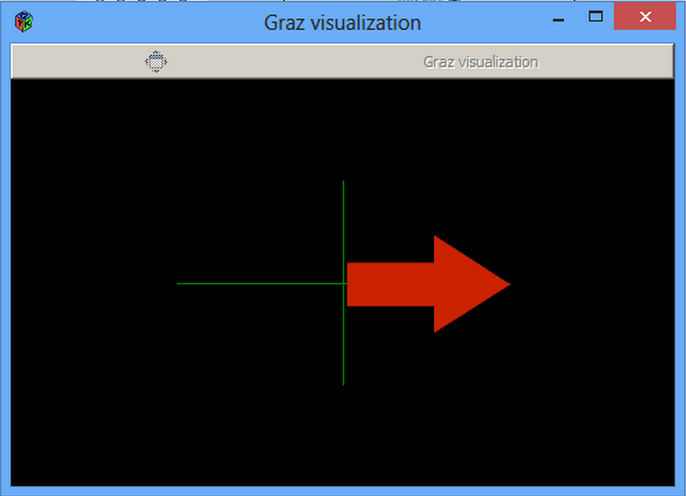
\includegraphics[height=7cm]{images/exempleAcquisition.png}
	\caption[Stimulation visuelle pour l'apprentissage.]{Stimulation visuelle pour l'apprentissage. 40 stimuli visuels sont présentés à l'utilisateur. Lorsque que celui-ci voit une flèche orientée vers la gauche, il doit penser à un mouvement de sa main gauche. Même exercice pour les flèches orientées vers la droite.}
	\label{acqui}
\end{figure}

\begin{figure}[h]
	\centering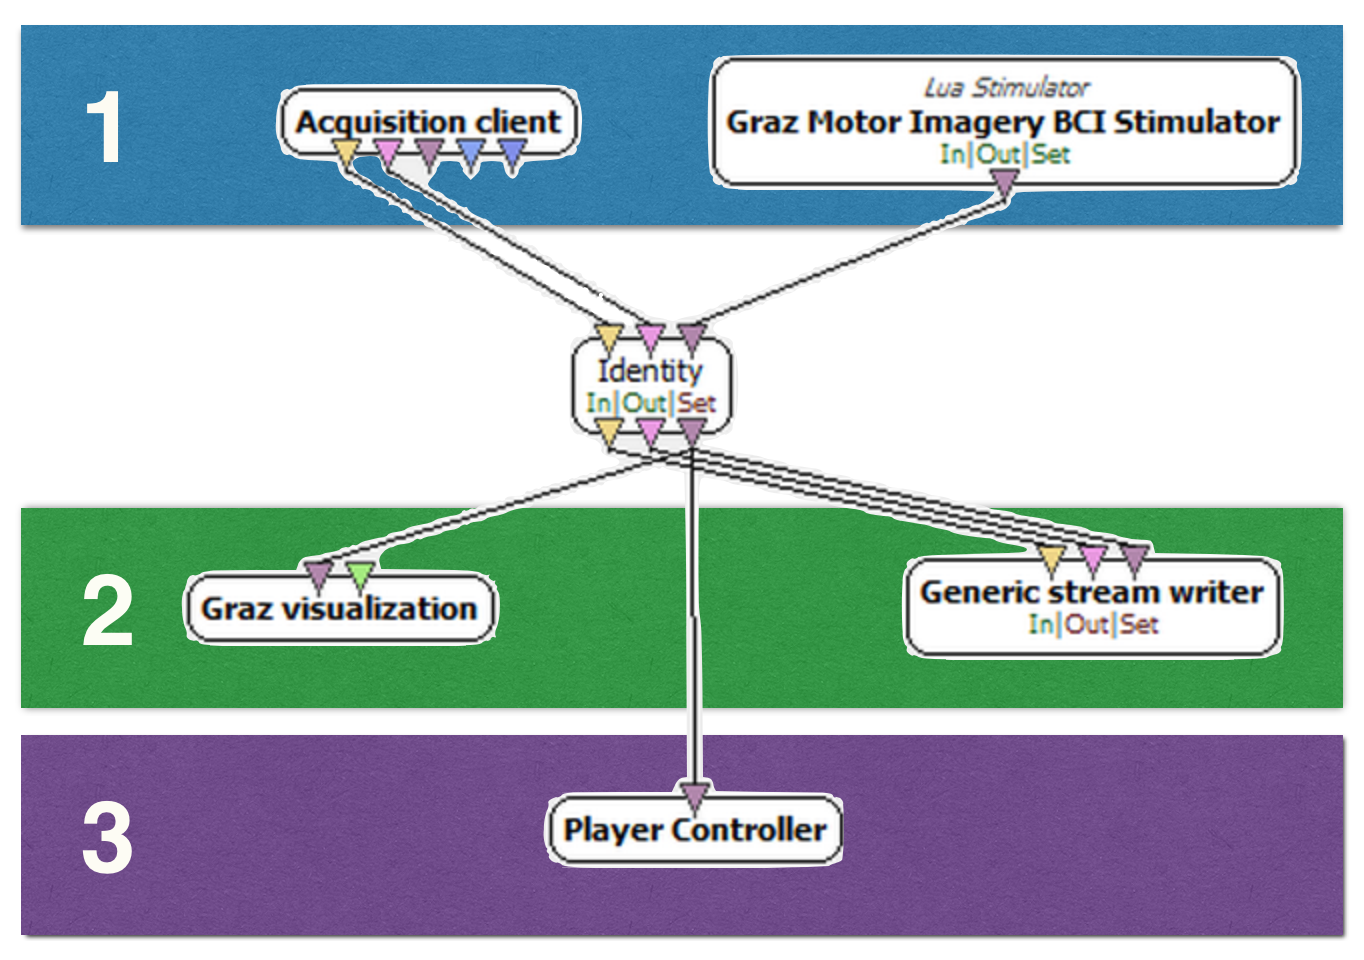
\includegraphics[height=9cm]{images/scenario1.png}
	\caption[Scénario 1 : Acquisition.]{Scénario 1 : Acquisition. Les signaux EEG sont acquis à partir du casque via le bloc "acquisition client". On génère des stimuli visuels grâce au script LUA contenu dans le bloc "Graz Motor Imagery BCI Simulator". Les stimuli sont affichés via le bloc "Graz Visualisation" et " Player Controller". Les données EEG sont quant à elles enregistrées avec le bloc "Generic Stream Writer", générant un fichier .ov}
	\label{scena1}
\end{figure}





\subsection{Scénario 2 : Entrainement du filtre spatial CSP}
\label{Subsection : 6.Scénario 2}
Ce scénario gère l'entrainement du filtre spatial de type CSP (partie \ref{Subsubsecton : 4.CSP})  qui permet de réduire le nombre de canaux (sorties des électrodes) à traiter (Figure \ref{scena2}). Celui-ci fournit en sortie un fichier .cfg. Il s'agit d'un fichier contenant l'ensemble des informations de configuration du filtre CSP (poids attribué à chaque canal).

\textbf{Étapes de déroulement du scénario (Figure \ref{scena2}) : }
\begin{enumerate}
	\item On récupère les signaux EEG bruts et les labels de stimulation enregistrés lors de l'exécution du scénario précédent. 
	\smallbreak
	\item On réalise un filtrage temporel des signaux EEG afin de ne conserver que les rythmes alpha et bêta du cerveau.
	\smallbreak
	\item On découpe les signaux EEG en plusieurs parties, dont leur durée correspond à la durée d'un stimulus visuel. Ces sections sont triées en deux catégories : les signaux correspondant à une réponse à un stimulus gauche (flèche orientée vers la gauche) et les signaux correspondant à une réponse à un stimulus droit (flèche orientée vers la droite).
	\smallbreak
	\item On envoie les deux catégories de signaux vers l'entraineur du filtre CSP.
\end{enumerate}

Il faut environ 8 secondes pour que l'ordinateur calcule les paramètres du filtre (il faut utiliser la fonction de lecture rapide). A la fin de l'exécution du scénario, un message sur le terminal nous informe de la bonne réalisation de la configuration du filtre spatial (Figure \ref{consoleCSP}).

\smallbreak
\textbf{Configuration du bloc "Generic Stream Reader" : }
\smallbreak
\begin{itemize}
	\item File Name .ov : Indiquer le chemin vers le fichier .ov généré lors de l'exécution du scénario précédent, afin de récupérer les signaux EEG bruts et les labels de stimulation correspondants.
	\smallbreak
\end{itemize}

\smallbreak
\textbf{Configuration du bloc "Temporal Filter" : }
\smallbreak
\begin{itemize}
	\item Type de filtre : Butterworth, Passe bande.
	\smallbreak
	\item Fréquences de coupure : 8Hz - 30Hz.
\end{itemize}

\smallbreak
\textbf{Configuration des blocs "Simulation Based Epoching" : }
\smallbreak
\begin{itemize}
	\item Epoch Duration : Se réfère à la durée d'un stimulus visuel produit par le script LUA, afin de découper le signal en plusieurs parties dont la durée correspond à celle du stimulus visuel associé. La durée est ici de 4 secondes.
	\smallbreak
	\item Epoch Offset : Se réfère à la durée entre deux stimuli visuels. La durée est ici de 0.5 secondes.
	\smallbreak
	\item Stimulation to epoch from : Associe les fragments des signaux découpés au label de stimulation. Dans notre cas, il s'agira du label "OVTK\_GDF\_Left" pour les fragments de signaux EEG correspondant aux stimuli de gauche et le label "OVTK\_GDF\_Right" pour les fragments de signaux EEG correspondant aux stimuli de droite.
\end{itemize}

\smallbreak
\textbf{Configuration du bloc "CSP Spatial Filter Trainer" : }
\smallbreak
\begin{itemize}
	\item Spatial Filter Configuration : Indiquer le chemin et le nom du fichier vers lequel le scénario doit enregistrer le fichier de configuration du CSP (extension .cfg). 
	\smallbreak
	\item Filter Dimension : Spécifie le nombre de sorties que l'on souhaite obtenir après le filtrage spatial.
\end{itemize}

\begin{figure}[h]
	\centering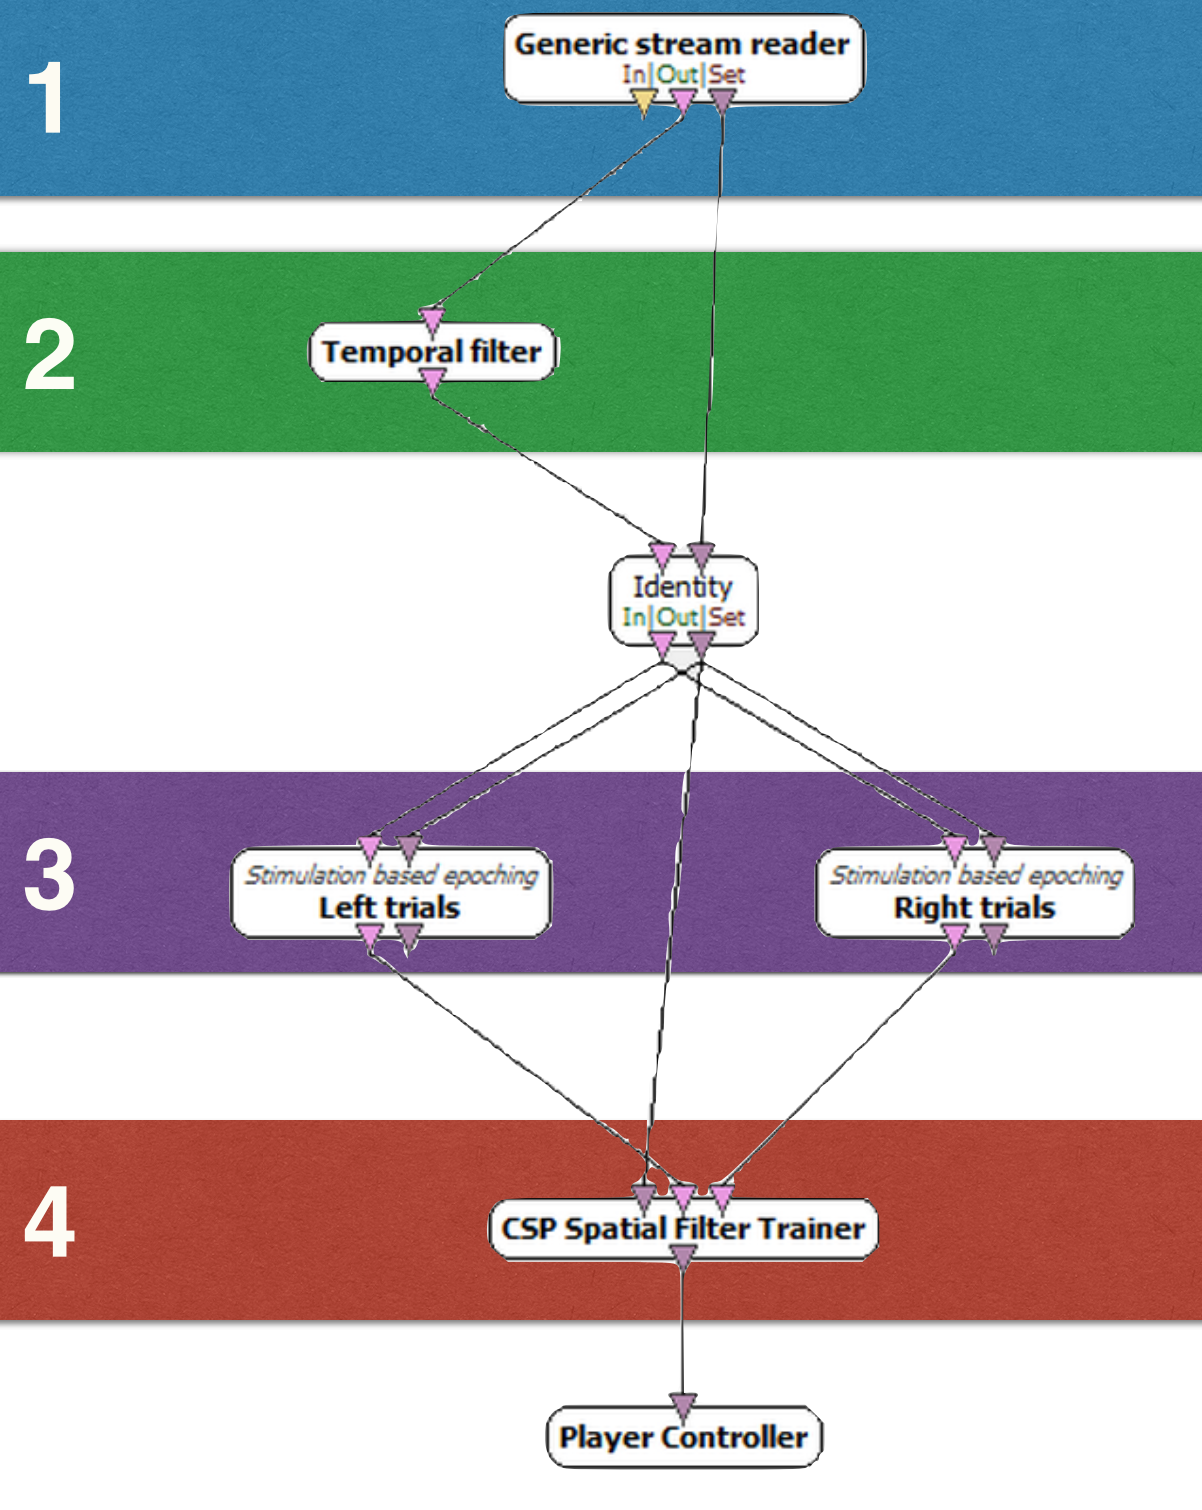
\includegraphics[height=13cm]{images/scenario2.png}
	\caption[Scénario 2 : Entrainement du filtre spatial]{Scénario 2 : Entrainement du filtre spatial. On récupère les données acquises à partir du scénario précédent (bloc "Generic Stream Reader"), puis on réalise un filtrage temporel des signaux EEG afin d'extraire les rythmes alpha et bêta. On découpe et on trie ensuite les signaux EEG en fonction des stimulations visuelles. On entraine le CSP à partir de ces signaux découpés.}
	\label{scena2}
\end{figure}

\begin{figure}[h]
	\centering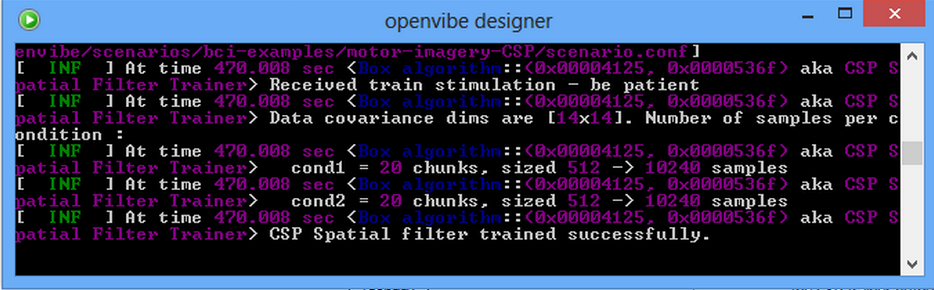
\includegraphics[height=4cm]{images/consoleCSP.png}
	\caption[Sortie console de l'entrainement du CSP]{Sortie console de l'entrainement du CSP. Lorsque l'entrainement du CSP est terminé, le message "CSP Spatial filter trained successfully" apparait.}
	\label{consoleCSP}
\end{figure}





\subsection{Scénario 3 : Entrainement du classificateur}
\label{Subsection : 6.Scénario 3}
Ce scénario sert à entrainer le classificateur LDA (partie \ref{Subsubsection : 4.Linear Discriminant Analysis}) afin que la liaison cerveau-ordinateur soit en mesure de classer les signaux EEG reçus en deux catégories : les signaux correspondants à la pensée de la main gauche, et ceux correspondants à la main droite (Figure \ref{scena3}). Le classificateur se base sur les données acquises lors de l'utilisation du premier scénario et utilise ainsi le fichier .ov qui a été généré. Il utilise également le fichier de configuration obtenu avec l'entrainement du CSP. Le scénario fournit en sortie un fichier .cfg. Il s'agit d'un fichier contenant l'ensemble des informations de configuration du classificateur LDA (Hyperplan et équation du plan).

\smallbreak
\textbf{Étapes de déroulement du scénario (Figure \ref{scena3}) : }
\smallbreak
\begin{enumerate}
	\item On récupère les signaux EEG bruts et les labels de stimulation enregistrés lors de l'exécution du scénario 1. 
	\smallbreak
	\item On réalise un filtrage temporel des signaux EEG afin de ne conserver que les rythmes alpha et bêta du cerveau.
	\smallbreak
	\item On réalise un filtrage spatial de type CSP, à partir de la configuration obtenue dans le scénario précédent. On obtient donc en sortie les canaux sélectionnés et pondérés par le filtre.
	\smallbreak
	\item On découpe les signaux EEG en plusieurs parties, dont leur durée correspond à la durée d'un stimulus visuel. Ces sections sont triées en deux catégories : les signaux correspondant à une réponse à un stimulus gauche (flèche orientée vers la gauche) et les signaux correspondant à une réponse à un stimulus droit (flèche orientée vers la droite).
	\smallbreak
	\item On recoupe de nouveau ces signaux afin d'obtenir des éléments ayant une durée de 1 seconde.
	\smallbreak
	\item On réalise une analyse spectrale en décomposant le signal en série de Fourier. 
	\smallbreak
	\item On place les spectres des signaux dans un vecteur caractéristique.
	\smallbreak
	\item On entraîne le classificateur. 
\end{enumerate}

À la fin de cette opération, un indice de performance est donné dans la console d'OpenViBE. Cet indice doit être supérieur à 65\% si l'on veut espérer obtenir des résultats cohérents lorsque la liaison cerveau-ordinateur fonctionnera en temps réel, i.e. lors de l'execution du scénario 4 (Figure \ref{consoleClassifier}). Dans le cas contraire, il faut recommencer là partir de la phase d'acquisition (Scénario 1) pour obtenir un meilleur résultat.

\smallbreak
\textbf{Configuration du bloc "Generic Stream Reader" : }
\smallbreak
\begin{itemize}
	\item File Name .ov : Indiquer le chemin vers le fichier .ov généré lors de l'exécution du scénario 1, afin de récupérer les signaux EEG bruts et les labels de stimulation correspondants.
	\smallbreak
\end{itemize}

\smallbreak
\textbf{Configuration du bloc "Temporal Filter" : }
\smallbreak
\begin{itemize}
	\item Type de filtre : Butterworth, Passe bande.
	\smallbreak
	\item Fréquences de coupure : 8Hz - 30Hz.
\end{itemize}

\smallbreak
\textbf{Configuration du bloc "CSP Spatial Filter" : }
\smallbreak
\begin{itemize}
	\item Sélectionner l'option "Override setting with configuration file" puis indiquer le chemin vers le fichier de configuration du CSP généré lors du scénario précédent. Les paramètres "Spatial Filter Coefficients", "Number of Output Channels" et "Number of Input Channels" se configurent alors automatiquement. 
\end{itemize}

\smallbreak
\textbf{Configuration des blocs "Simulation Based Epoching" : }
\smallbreak
\begin{itemize}
	\item Epoch Duration : Se réfère à la durée d'un stimulus visuel produit par le script LUA, afin de découper le signal en plus parties dont la durée correspond à celle du stimulus visuel associé. La durée est ici de 4 secondes.
	\smallbreak
	\item Epoch Offset : Se réfère à la durée entre deux stimuli visuels. La durée est ici de 0.5 secondes.
	\smallbreak
	\item Stimulation to epoch from : associe les fragments de signaux découpés au label de stimulation. Dans notre cas, il s'agira du label "OVTK\_GDF\_Left" pour les fragments de signaux EEG correspondant aux stimuli de gauche et le label "OVTK\_GDF\_Right" pour les fragments de signaux EEG correspondant aux stimuli de droite.
\end{itemize}

\smallbreak
\textbf{Configuration du bloc "Time Based Epoching" : }
\smallbreak
\begin{itemize}
	\item Epoch 1 duration : Correspond à la durée des tranches de signaux. 1 seconde dans le cas présent.
	\smallbreak
	\item Epoch 1 intervals : Intervalle de temps entre chaque tranche de signal. 0.0625 secondes dans le cas présent. 
\end{itemize}

\smallbreak
\textbf{Configuration du bloc "Spectral analysis (FFT)" : }
\smallbreak
\begin{itemize}
	\item Spectral components : Permet de sélectionner la composante spectrale analysée. On souhaite ici utiliser le spectre d'amplitude du signal. 
\end{itemize}

\smallbreak
\textbf{Configuration du bloc "Spectrum Average" : }
\smallbreak
\begin{itemize}
	\item Ne requière pas de configuration particulière.
\end{itemize}

\smallbreak
\textbf{Configuration du bloc "Classifier trainer" : }
\smallbreak
\begin{itemize}
	\item Train Trigger : Permet de sélectionner le drapeau permettant de démarrer l'entrainement du classificateur. Il s'agit ici du drapeau "OVTK\_Stimulationid\_Train qui est généré par les données de stimulation provenant du bloc "Generic stream reader".
	\smallbreak
	\item Filename to save configuration to : Permet de sélectionner le répertoire et le nom sous lequel enregistrer le fichier de configuration du classificateur (extension .cfg).
	\smallbreak
	\item Class 1 label : Sélectionne le label de la classe 1. Il s'agira ici du label utilisé pour la stimulation gauche (flèche orientée à gauche) "OVTK\_GDF\_Left".
	\smallbreak
	\item Class 2 label : Sélectionne le label de la classe 2. Il s'agira ici du label utilisé pour la stimulation droite (flèche orientée à droite) "OVTK\_GDF\_Right".
	\smallbreak 
	\item Algorithm to use : Permet de sélectionner le type de classification à réaliser (LDA ou SVM). On décide ici d'utiliser un classificateur LDA.
\end{itemize}

\begin{figure}[h]
	\centering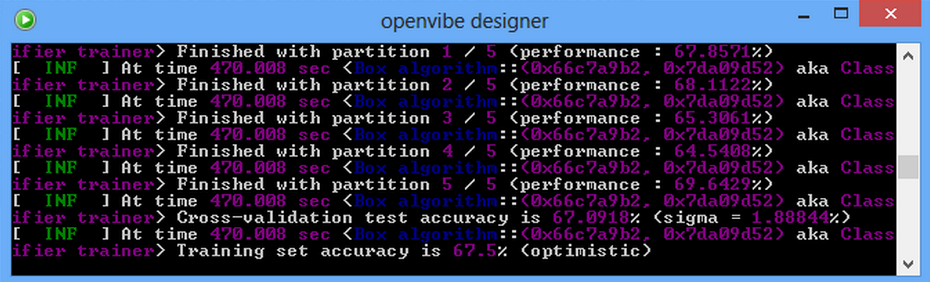
\includegraphics[height=4cm]{images/consoleClassifier.png}
	\caption[Sortie console résultant de l'entrainement du classificateur.]{Sortie console résultant de l'entrainement du classificateur. Une valeur correspondant en pourcentage à la précision de l'entraînement de la classification nous est fournie.}
	\label{consoleClassifier}
\end{figure}

\begin{figure}[h]
	\centering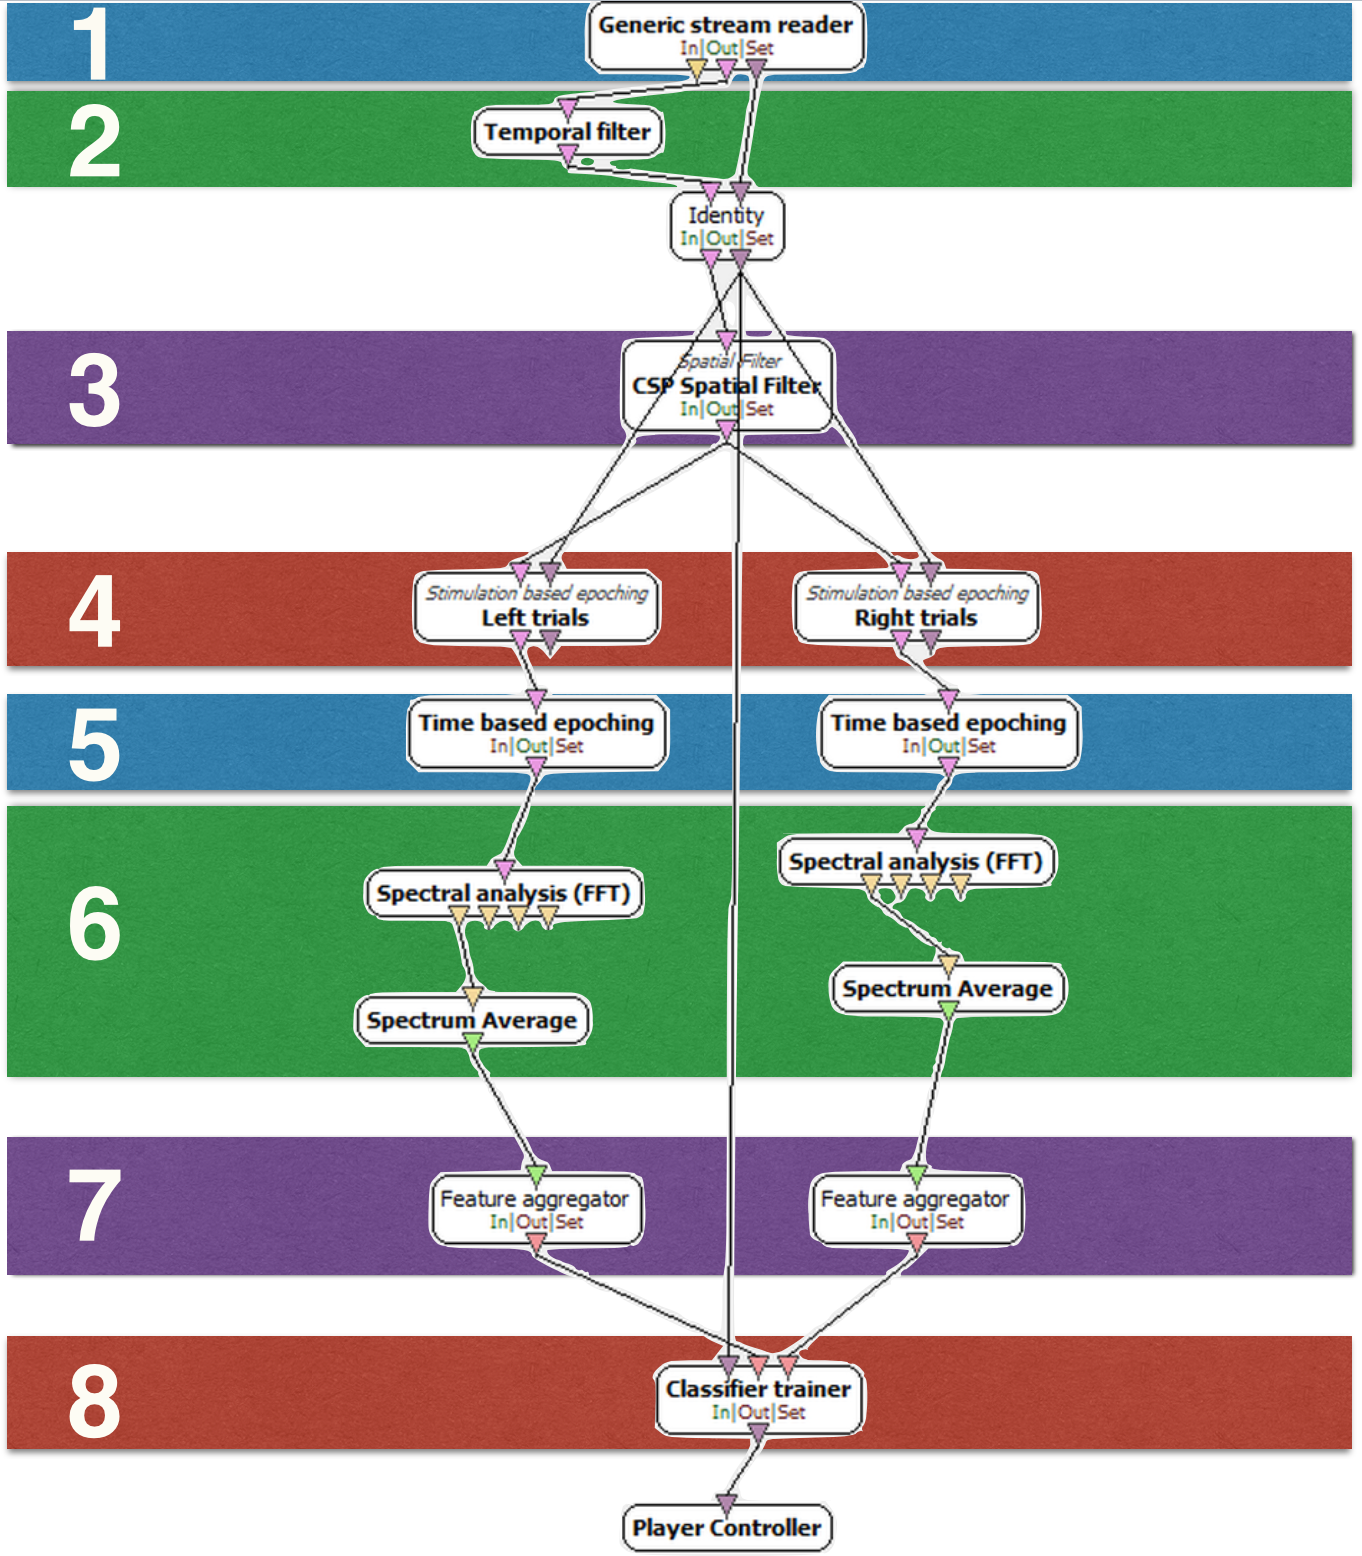
\includegraphics[height=16cm]{images/scenario3.png}
	\caption[Scénario 3 : Entrainement du classificateur]{Scénario 3 : Entrainement du classificateur. A partir des signaux acquis lors du scénario 1, on vient entrainer le classificateur en vu de l'utiliser pour le scénario 4 (temps réel). Pour cela, on commence par filtrer des signaux d'entrée afin d'extraire les signaux alpha et bêta du cerveau. Puis on réalise un filtrage spatial grâce au filtre CSP entrainé lors du scénario précédent. Enfin on effectue un analyse spectral des signaux filtrés pour les présenter en entrée de l'entraineur du classificateur.}
	\label{scena3}
\end{figure}








\subsection{Scénario 4 : Utilisation en temps réel de l'interface}
\label{Subsection : 6.Scénario 4}
Ce scénario permet d'utiliser la liaison cerveau-ordinateur en temps réel. Il s'appuie sur les configurations effectuées grâce aux scénarios précédents, i.e. le filtre spatial CSP et classificateur LDA (Figure \ref{scena4}). On place dans le scénario un certain nombre de blocs permettant de visualiser les résultats obtenus ("Signal display, "Power spectrum display", "Post CSP display", "Graz Visualisation").

\textbf{Étapes de déroulement du scénario (Figure \ref{scena3}) : }
\begin{enumerate}
	\item On récupère les signaux EEG  à partir du casque EPOC, en temps réel (Figure : \ref{xpBrut}).
	\smallbreak 
	\item On réalise un filtrage temporel des signaux EEG afin de ne conserver que les rythmes alpha et bêta du cerveau (Figure : \ref{xpFiltered}).
	\smallbreak
	\item On réalise un filtrage spatial de type CSP, à partir de la configuration obtenue dans le scénario 2. On obtient donc en sortie les canaux sélectionnés et pondérés par le filtre (Figure : 	\ref{xpCsp}).
	\smallbreak
	\item On découpe les signaux afin d'obtenir des tranches de signal ayant une durée de 1 seconde.
	\smallbreak
	\item On réalise une analyse spectrale en décomposant le signal en série de Fourier (Figure : \ref{xpPowerSpectrum}).
	\smallbreak
	\item On place les spectres des signaux dans un vecteur caractéristique.
	\smallbreak
	\item On réalise la classification des données à partir du classificateur entrainé grâce au scénario précédent. On obtient donc en sortie l'estimation du système quant à la pensée de l'utilisateur (Figure : \ref{online}).
\end{enumerate}

\smallbreak
\textbf{Configuration du bloc "Acquisition Client" : }
\smallbreak
\begin{itemize}
	\item Acquisition Server HostName : "\${AcquisitionServer\_HostName}".
	\smallbreak
	\item Acquisition Server Port : Port de connexion correspondant au casque Epoc. Valeur par défaut 1024.
\end{itemize}

\smallbreak
\textbf{Configuration du bloc "Temporal Filter" : }
\smallbreak
\begin{itemize}
	\item Type de filtre : Butterworth, Passe bande.
	\smallbreak
	\item Fréquences de coupure : 8Hz - 30Hz.
\end{itemize}

\smallbreak
\textbf{Configuration du bloc "CSP Spatial Filter" : }
\smallbreak
\begin{itemize}
	\item Sélectionner l'option "Override setting with configuration file" puis indiquer le chemin vers le fichier de configuration du CSP généré lors du scénario précédent. Les paramètres "Spatial Filter Coefficients", "Number of Output Channels" et "Number of Input Channels" se configurent alors automatiquement. 
\end{itemize}

\smallbreak
\textbf{Configuration du bloc "Time Based Epoching" : }
\smallbreak
\begin{itemize}
	\item Epoch 1 duration : Correspond à la durée des tranches de signaux. 1 seconde dans le cas présent.
	\smallbreak
	\item Epoch 1 intervals : Intervalle de temps entre chaque tranches de signal. 0.0625 secondes dans le cas présent. 
\end{itemize}

\smallbreak
\textbf{Configuration du bloc "Spectral analysis (FFT)" : }
\smallbreak
\begin{itemize}
	\item Spectral components : Permet de sélectionner la composante spectrale analysée. On souhaite ici utiliser le spectre d'amplitude du signal. 
\end{itemize}

\smallbreak
\textbf{Configuration du bloc "Spectrum average" : }
\smallbreak
\begin{itemize}
	\item Ne requière pas de configuration particulière.
\end{itemize}

\smallbreak
\textbf{Configuration du bloc "Classifier processor" : }
\smallbreak
\begin{itemize}
	\item Filename to load configuration from : Indiquer le chemin vers le fichier de configuration généré lors de l'exécution du scénario précédent.
\end{itemize}

\begin{figure}[h]
	\centering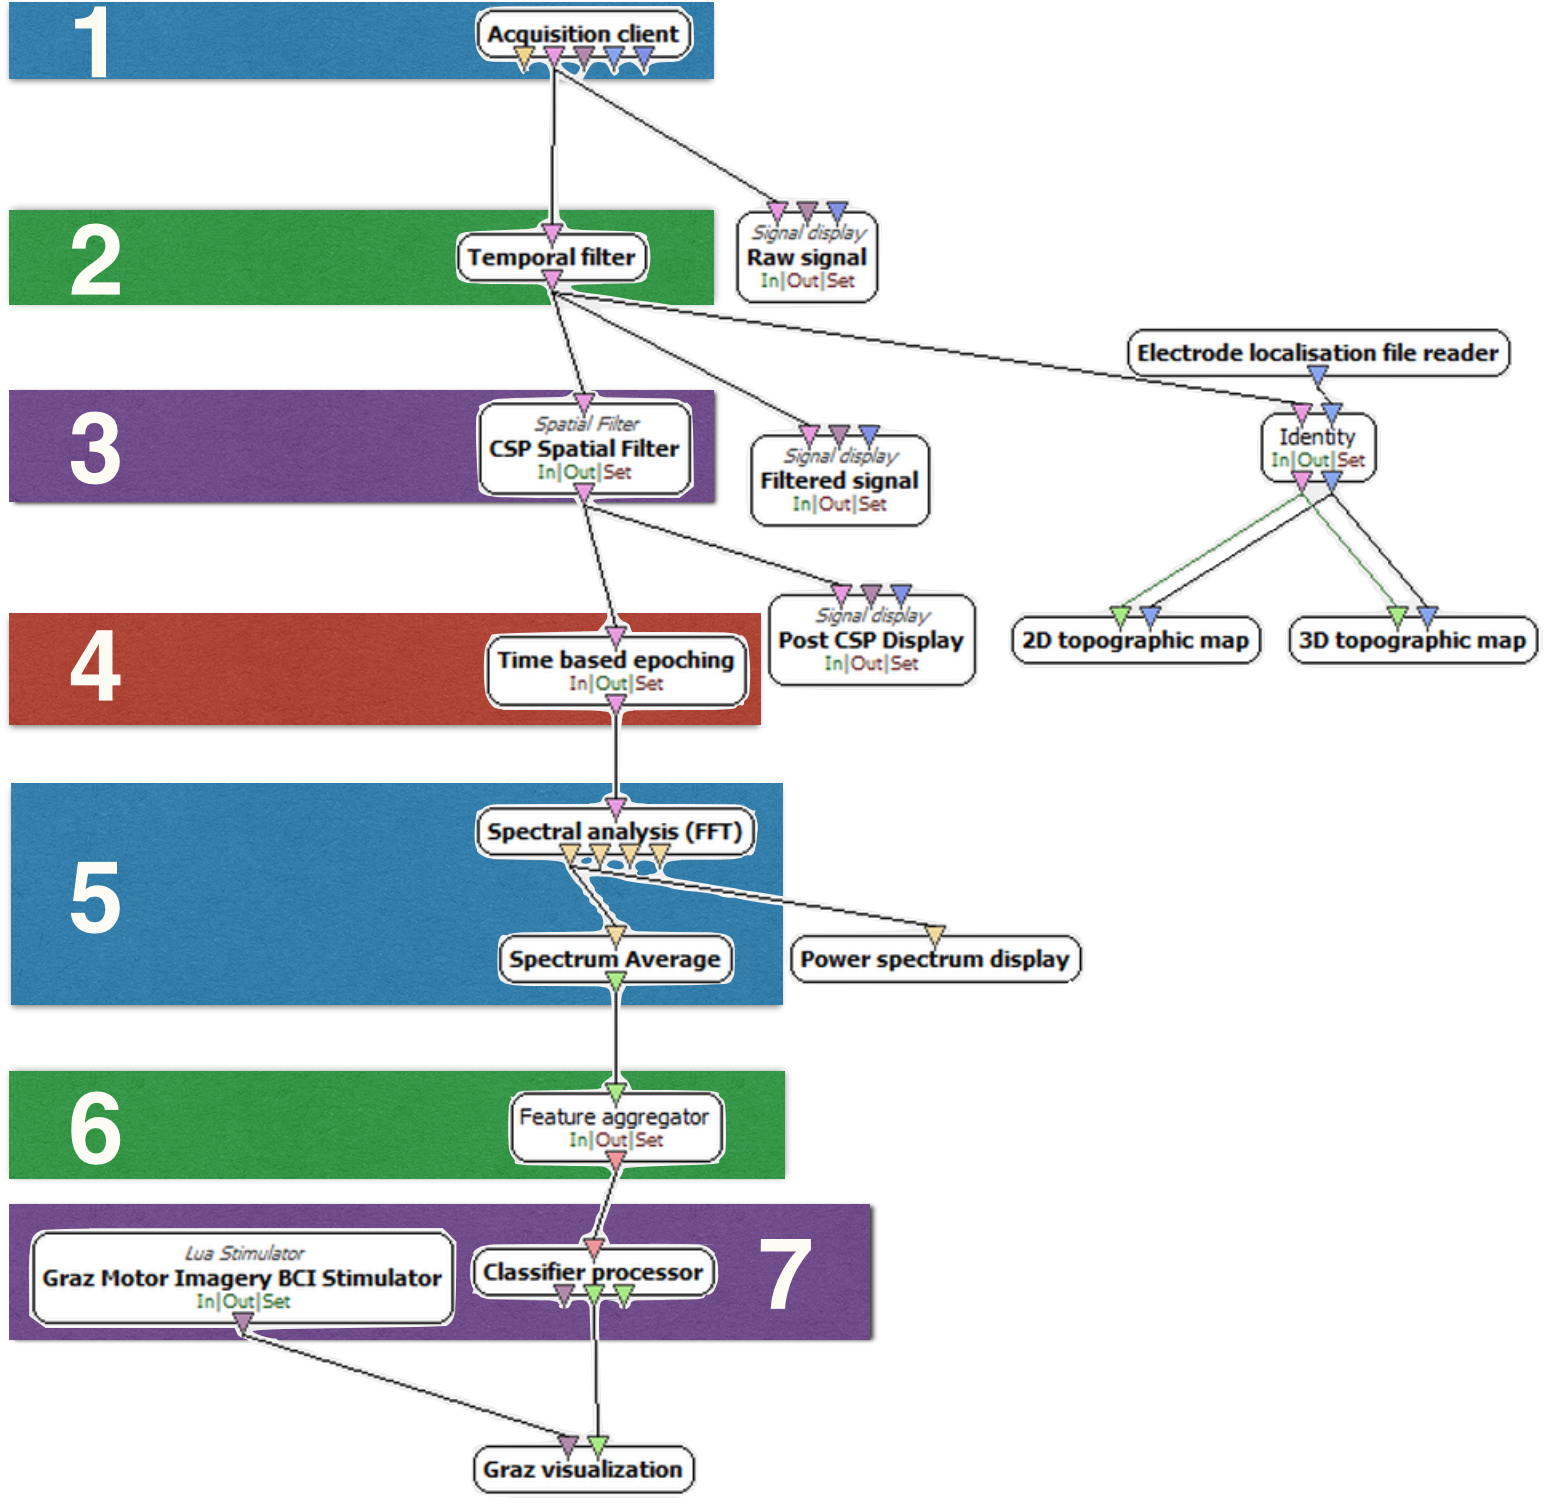
\includegraphics[height=16cm]{images/scenario4.png}
	\caption[Scénario 4 : Utilisation en temps réel]{Scénario 4 : Utilisation en temps réel. Celui-ci permet d'utiliser la liaison cerveau-ordinateur en temps réel. Pour cela, on enregistre en entrée les signaux provenant en temps réel du casque (bloc "acquisition client"). On effectue par la suite un filtrage temporel afin d'extraire les rythmes alpha et bêta du cerveau. On réalise à partir de ces rythmes un filtrage CSP afin de réduire le nombre de signaux en sortie. Une analyse spectrale est ensuite réalisée afin d'effectuer une classification LDA. Les données sont visualisées via les différents bloc de visualisation.}
	\label{scena4}
\end{figure}





\section {Résultats obtenus et analyse}
\label{Section : 6.Résultats obtenus et analyse}
Au départ, notre première expérience utilisait un filtre statique de type Laplacien. Or, les résultats obtenus n'étaient pas satisfaisant (55\% de performances environ). Après remplacement du filtre statique par un filtre spatial par apprentissage de type CSP, on obtient de meilleurs performances. (75 à 80 \% de performance avec le filtre CSP).

Deux facteurs principaux altèrent la qualité des résultats :
\smallbreak
\begin{itemize}
	\item \textbf{Qualité des signaux d'entrée.} Un mauvais positionnement du casque sur le crâne ou une mauvaise hydratation des électrodes peut réduire la qualité des signaux entrant dans le système, réduisant ainsi la qualité des résultats.
	\smallbreak
	\item \textbf{Concentration de l'utilisateur.}  L'exécution du premier scénario nécessite une concentration importante de l'utilisateur. En effet, si celui-ci ne se concentre pas suffisamment sur les stimuli visuels et sur sa représentation visuelle du mouvement de ses main, la qualité de la classification sera altérée. De même si l'individu parle ou bouge durant l'acquisition des données.
\end{itemize}


\begin{figure}[h]
	\centering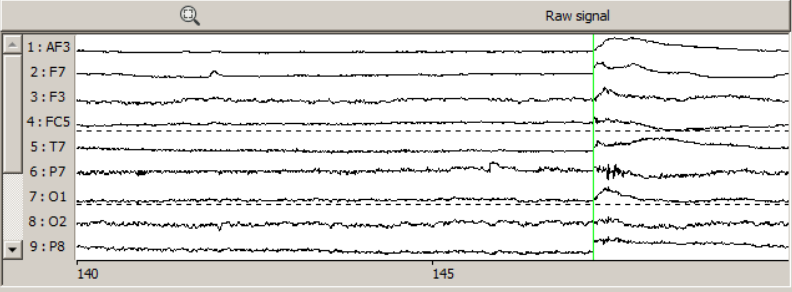
\includegraphics[height=4cm]{images/xpRawSignal.png}
	\caption[Signaux bruts observés en sortie du casque Emotiv]{Signaux bruts observés en sortie du casque Emotiv, sur les 14 canaux (électrodes).}
	\label{xpBrut}
\end{figure}

\begin{figure}[h]
	\centering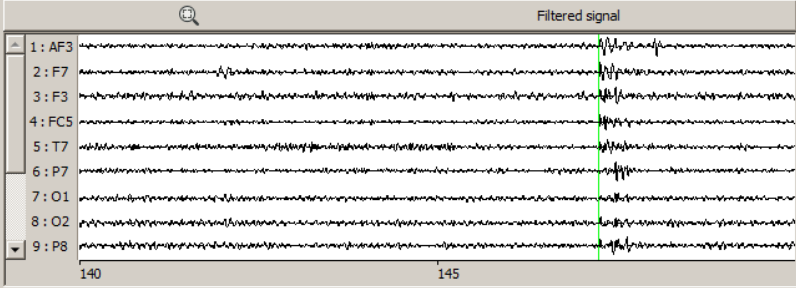
\includegraphics[height=4cm]{images/xpFilteredSignal.png}
	\caption[Signaux filtrés]{Signaux filtrés temporellement afin d'extraire les rythmes alpha et bêta du cerveau.}
	\label{xpFiltered}
\end{figure}

\begin{figure}[h]
	\centering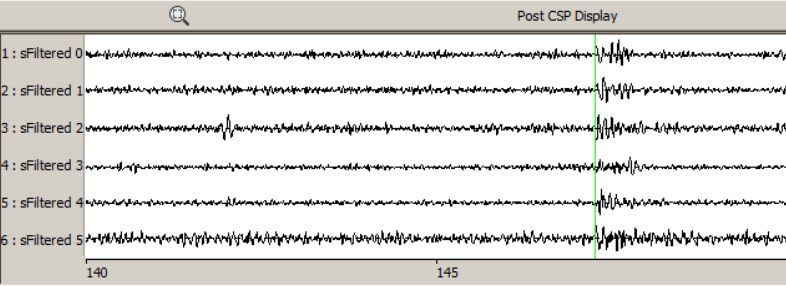
\includegraphics[height=4cm]{images/xpCsp.png}
	\caption[Réduction du nombre de sorties grâce au filtrage CSP]{Réduction du nombre de sorties grâce au filtrage CSP. On passe de 14 entrées à 6 sorties.}
	\label{xpCsp}
\end{figure}

\begin{figure}[h]
	\centering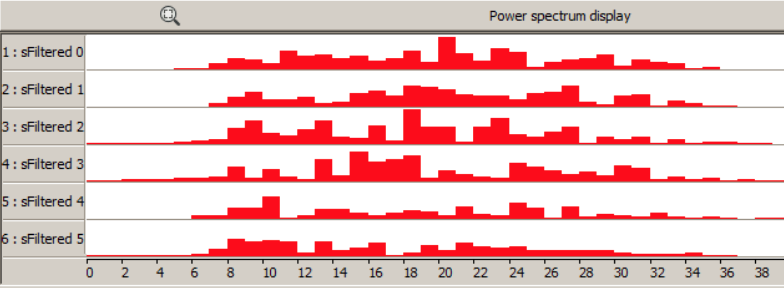
\includegraphics[height=4cm]{images/xpPowerSpectrum.png}
	\caption[Analyse spectrale des signaux]{Analyse spectrale des signaux via une transformation de Fourier.}
	\label{xpPowerSpectrum}
\end{figure}

\newpage
\begin{figure}[h]
	\centering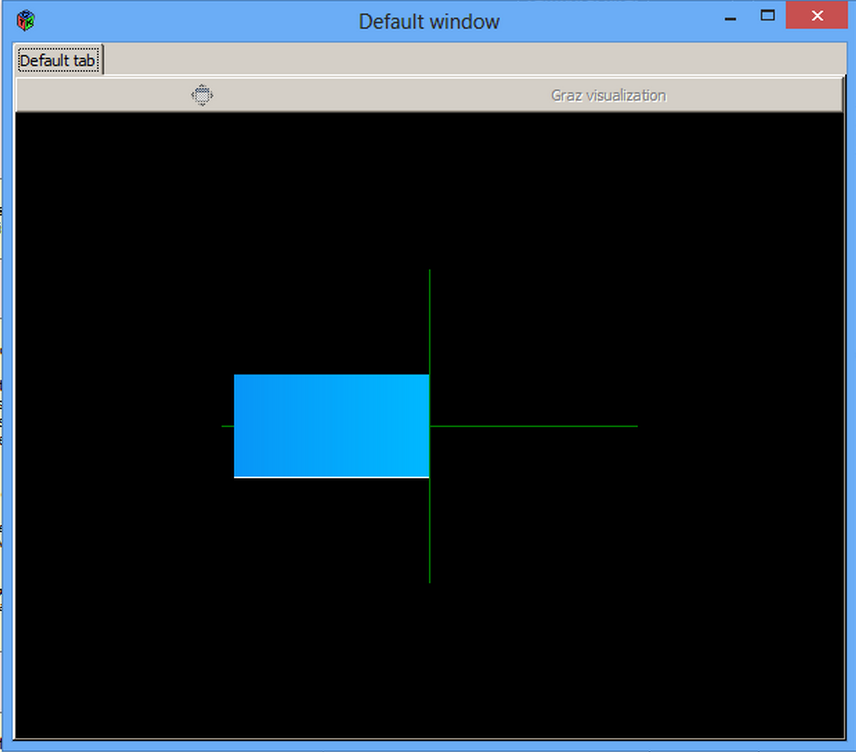
\includegraphics[height=10cm]{images/online.png}
	\caption[Sortie visuelle temps réel après classification]{Sortie visuelle temps réel après classification. La direction du curseur bleu correspond à la pensée de l'utilisateur : Si le curseur se dirige vers la gauche, cela signifie que le système estime que la personne pense à un mouvement de sa main gauche. Si au contraire le curseur se dirige vers la droite, cela signifie que le système estime que la personne pense à un mouvement de sa main droite. Plus le curseur s'éloigne du centre de l'image, plus la certitude du système est élevée.}
	\label{online}
\end{figure}